\documentclass[11pt]{article}

\usepackage[margin=1in]{geometry}
\usepackage{graphicx}
\usepackage{booktabs}
\usepackage{amsmath}
\usepackage{hyperref}
\usepackage{caption}
\usepackage{float}

\title{Phase 4: Evaluation, Synthesis \& Reporting \\
\large Pan-Cancer RNA-Seq Intrinsic Dimensionality Project}
\author{}
\date{\today}

\begin{document}
\maketitle

\begin{abstract}
This report synthesizes Phases 1--3 of ``When 20,531 Dimensions Hide a
Handful of Truths'' into a single coherent account of the gap between the
ambient dimension $d = 20{,}531$ (analysis dimension $d = 20{,}264$ after
removing $267$ zero-variance genes, Phase 1) and the intrinsic dimension of
the $n = 801$-sample TCGA Pan-Cancer expression manifold. Four independent
estimates of that intrinsic dimension are reconciled: the Grassberger--Procaccia
correlation dimension ($D_2 = 7.73$), the Levina--Bickel $k$-NN MLE mean
($29.36$ across $k \in \{5,10,20\}$), the count of Marchenko--Pastur spectral
outliers on the top-$2{,}000$-gene correlation matrix ($27$), and the
Kaiser-criterion PCA elbow ($100$ of $392$ components needed for $90\%$
variance). We show these do not disagree by accident: each probes a
different notion of ``dimension'' (local neighborhood scaling, local
maximum-likelihood neighbor statistics, global but signal-filtered linear
variance, global unfiltered linear variance), and their strict ordering
$D_2 < \text{MP outliers} \approx k\text{NN-MLE} \ll \text{Kaiser} \ll
\text{PCA@90\%}$ is itself evidence for -- not against -- a genuinely
low-dimensional, but nonlinearly embedded, manifold. We further show that
this reconciles Phase 3's central visual puzzle: $3$ linear principal
components capture only $26.64\%$ of variance and yield only partial
cancer-type separation, while nonlinear t-SNE/UMAP embeddings of the same
data (after linear PCA preprocessing to $50$ components) recover
near-perfect five-cluster structure at every hyperparameter setting tested.
A consolidated table collects every diagnostic computed across Phases 2--3
-- intrinsic-dimension estimators against Gaussian-noise and linear-manifold
baselines, PCA variance cutoffs, Johnson--Lindenstrauss empirical distortion
($\bar\rho = 0.9996$, $100\%$ of pairs within the theoretical $\varepsilon =
0.2$ bound), and Mahalanobis outlier counts ($0$ of $801$ samples at a
$97.5\%$ $\chi^2_{800}$ threshold, the rank of the estimator). We close with an explicit discussion of
methodological limitations (COAD's $n \approx 78$, TCGA multi-center batch
effects, and gene co-expression's violation of the i.i.d.\ assumptions
underlying Marchenko--Pastur and the Laurent--Massart concentration bound)
and concrete next steps given additional compute.
\end{abstract}

\section{Introduction}

Phases 1--3 each answered a narrower question: Phase 1 established a
justified preprocessing pipeline; Phase 2 produced three independent,
numerically calibrated estimates of intrinsic dimension; Phase 3 visualized
the resulting manifold and stress-tested four theoretical high-dimensional
phenomena against it. None of those phases, individually, answers the
project's founding question -- does the estimated number of ``true degrees
of freedom'' actually explain the geometric and visual behavior observed?
This phase closes that loop. Section~\ref{sec:synthesis} builds a single
mathematical argument spanning Phases 2--3, explicitly reconciling every
pairwise disagreement between the four independent dimension estimates
computed across the project and explaining why linear PCA needs far more
components than any of them to achieve visual cluster separation.
Section~\ref{sec:summary-table} consolidates every quantitative diagnostic
from Phases 1--3 into one table. Section~\ref{sec:limitations} states the
statistical limitations that qualify every claim made in this project.
Section~\ref{sec:future-work} states concrete next steps given more time or
compute.

\section{Synthesis: Reconciling Ambient, Intrinsic, and Visual Dimensionality}
\label{sec:synthesis}

\subsection{Four Independent Estimates, One Manifold}

Phase 2 established three estimators of intrinsic dimension on the
standardized, zero-variance-filtered matrix ($n=801$, $d=20{,}264$):
\begin{align}
D_2 &= \frac{d \log C(r)}{d \log r}\bigg|_{r \in [r_{\min}, r_{\max}]},
\qquad C(r) = \frac{2}{N(N-1)} \sum_{i<j} \mathbb{1}\left[\lVert x_i - x_j \rVert < r\right],
\label{eq:d2-recap}\\
m_k(x_i) &= \left[\frac{1}{k-2}\sum_{j=1}^{k-1} \ln\frac{T_k(x_i)}{T_j(x_i)}\right]^{-1},
\label{eq:lb-recap}
\end{align}
giving $D_2 = 7.73$ (correlation dimension, Eq.~\ref{eq:d2-recap}) and a
$k$-NN MLE mean of $29.36$ across $k \in \{5,10,20\}$ (Levina--Bickel,
Eq.~\ref{eq:lb-recap}), against a Kaiser-criterion PCA elbow of $100$
components and $392$ components needed for $90\%$ cumulative linear
variance. Phase 3 then added a fourth, independent estimate: of the
$2{,}000$ eigenvalues of the top-$2{,}000$-gene correlation matrix, $27$
exceed the Marchenko--Pastur theoretical bulk edge $b = 6.662$ at aspect
ratio $\gamma = 2.500$ -- eigenvalues that cannot be explained by an
unstructured random matrix of matching shape and are therefore attributable
to genuine covariance structure, not noise.

These four numbers -- $7.73$, $27$, $29.36$, $100$ -- are not four attempts
at the same measurement that merely failed to agree; they are four
\emph{different} operational definitions of ``dimension,'' and their strict
ordering is itself informative:
\begin{itemize}
  \item $D_2$ (correlation dimension) is the most locally defined and the
  most negatively biased in a small-$n$, large-$d$ regime: at $n=801$, the
  scaling region identified for the real data spans only $5$ radii
  ($r \in [149.6, 156.5]$, Phase 2, Section~4), because pairwise distances
  in $20{,}264$ dimensions are sparse and concentrated (a phenomenon Phase 3
  itself quantifies directly -- Table~\ref{tab:consolidated}, distance
  concentration ratio $4.96$ at full dimension), starving the small-radius
  regime of the many-pair statistics the estimator needs. $D_2$ is
  therefore the most conservative (smallest) of the four estimates.
  \item The Marchenko--Pastur outlier count ($27$) and the $k$-NN MLE mean
  ($29.36$) are close to each other despite resting on entirely different
  machinery -- one a global eigenvalue threshold on a curated,
  variance-filtered $2{,}000$-gene subset, the other a local
  maximum-likelihood neighbor-ratio statistic on the full $20{,}264$-gene
  space -- which is itself a form of independent triangulation: two
  unrelated estimators, one local and one global-but-signal-restricted,
  converge on the same order of magnitude ($\approx 27$--$30$).
  \item The Kaiser elbow ($100$) and the $90\%$-variance threshold ($392$)
  are both computed on the \emph{full}, unfiltered $20{,}264$-gene matrix,
  where thousands of low-signal genes each contribute a small but nonzero
  amount of variance (biological subtype heterogeneity within each of the
  five cancer types, plus technical noise) that a linear, global,
  variance-based method cannot distinguish from genuine additional
  manifold curvature. Restricting to the top-$2{,}000$ variance-ranked
  genes (as the spectral analysis does) strips out most of this
  low-signal mass and the outlier count drops by roughly $4\times$ relative
  to the Kaiser elbow -- direct evidence that a substantial share of the
  Kaiser elbow's $100$ components is diffuse noise/heterogeneity variance
  rather than core manifold structure.
\end{itemize}

\subsection{Does Intrinsic Dimension Match the Components Needed for Visual Separation?}

The na\"ive expectation -- that if the manifold's intrinsic dimension is
single-to-low-double digits, then a similarly small number of principal
components should suffice to visually separate the five cancer types --
is falsified by Phase 3's own results, and this falsification is itself
the central finding this phase must reconcile.

\begin{figure}[H]
\centering
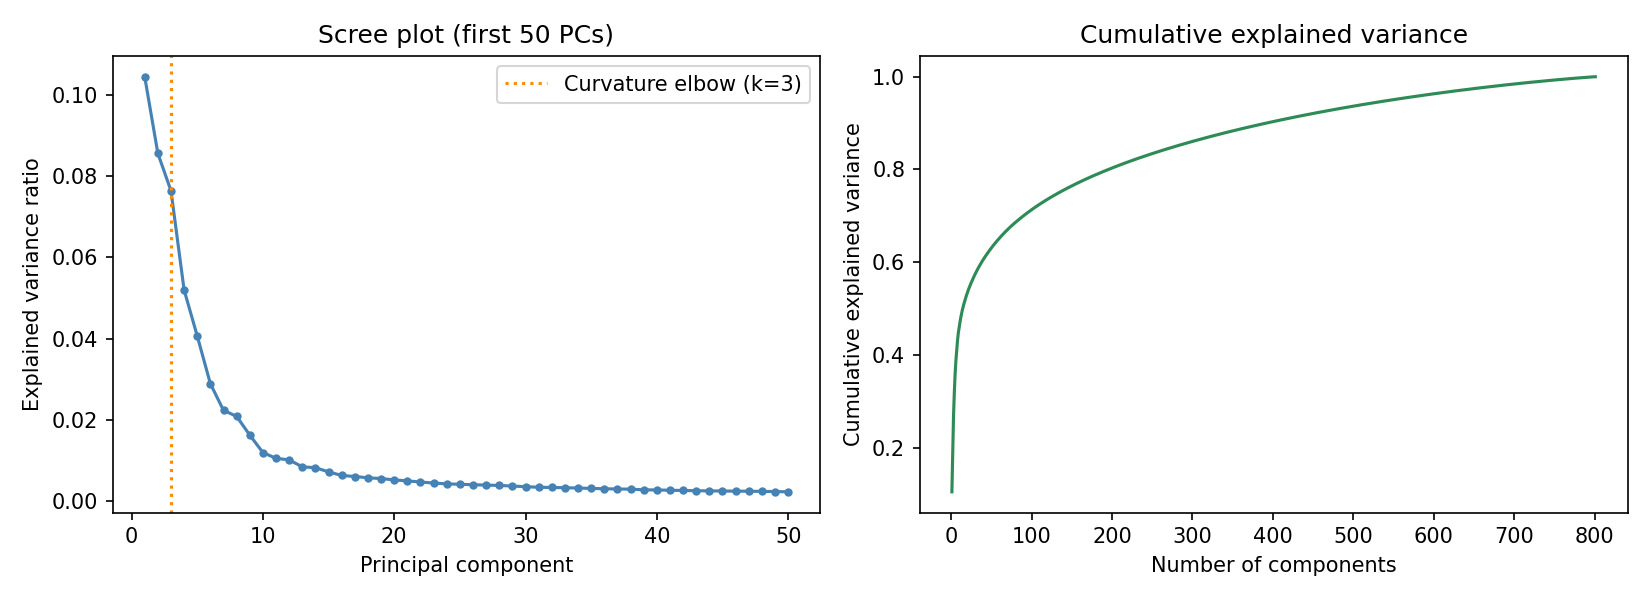
\includegraphics[width=0.95\textwidth]{../figures/scree_plot.png}
\caption{Scree plot of the real RNA-Seq covariance spectrum (reproduced
from Phase 2): per-component explained variance (first 50 PCs, left) and
cumulative explained variance across all 801 components (right). The
curve decays sharply within the first $\sim 10$ components but is not
exhausted until a long, shallow tail spanning hundreds of further
components.}
\label{fig:scree}
\end{figure}

Figure~\ref{fig:scree} shows why: the eigenvalue spectrum decays sharply
but continuously, with no sharp cutoff at any single-digit or low-double-digit
component index. The first $3$ components -- the maximum practically
visualizable in a static 2D/3D scatter plot -- together explain only
$26.64\%$ of total variance (Phase 3, Section~4.1), and while KIRC and COAD
form visually distinct clusters along PC1/PC2, BRCA, LUAD, and PRAD show
only partial linear separability with substantial overlap. Yet t-SNE and
UMAP, applied to the \emph{same} underlying data (linearly PCA-reduced to
$50$ dimensions as a preprocessing step, not more), recover five
essentially pure, well-separated clusters at every hyperparameter setting
tested (Phase 3, Section~4.1) -- see Figure~\ref{fig:corrdim} for the
correlation-dimension evidence of local, non-Euclidean scaling that
motivates why this is expected.

\begin{figure}[H]
\centering
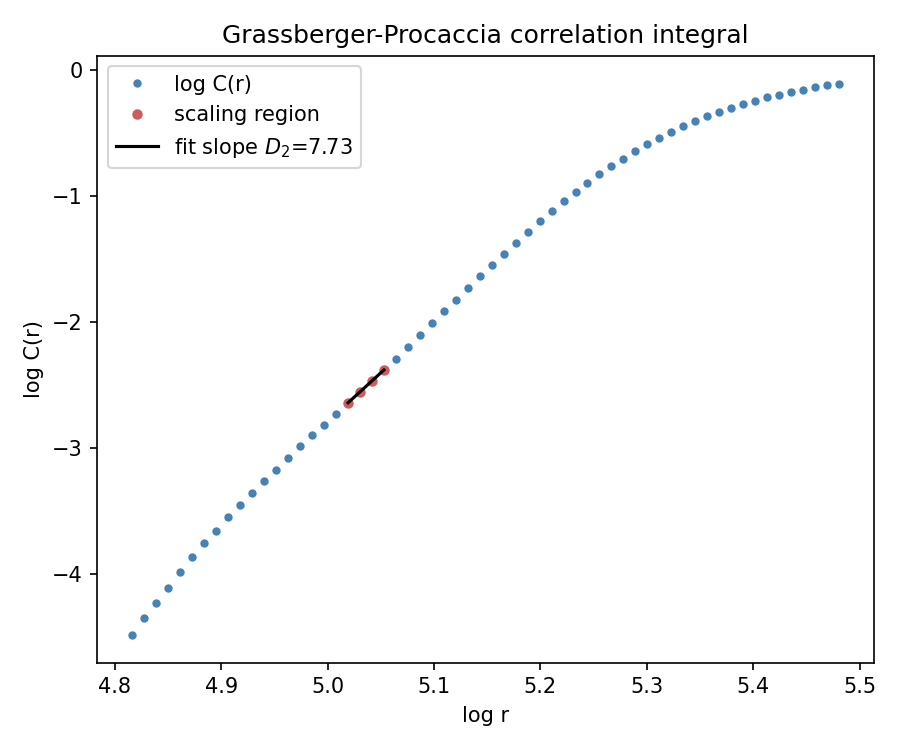
\includegraphics[width=0.7\textwidth]{../figures/log_log_correlation.png}
\caption{Log-log Grassberger--Procaccia correlation integral $C(r)$ for the
real RNA-Seq data (reproduced from Phase 2), with the automatically
detected scaling region and fitted slope $D_2 = 7.73$ highlighted. The
curve is smoothly convex with no long linear stretch, consistent with a
curved rather than flat local manifold structure.}
\label{fig:corrdim}
\end{figure}

The resolution is that ``intrinsic dimension'' as estimated by $D_2$,
$k$-NN MLE, and the spectral-outlier count measures the \emph{local
degrees of freedom} of the data-generating manifold -- how many coordinates
are needed to parameterize a small neighborhood of any given sample -- and
says nothing about whether that manifold is \emph{linearly flat}. A
manifold can have intrinsic dimension $7$ while being so curved through the
ambient space that no $7$-, or even $100$-dimensional, linear subspace
captures it via orthogonal projection with clean class separation: PCA, as
a purely linear method, must spend components on \emph{unfolding} curvature,
not only on tracking genuine degrees of freedom (Phase 2, Section~5). This
is precisely why the Kaiser elbow ($100$) and $90\%$-variance threshold
($392$) so greatly exceed $D_2$ and the $k$-NN MLE mean: they are answering
a different, strictly harder question (``how many \emph{linear} directions
are needed'') than intrinsic-dimension estimators answer (``how many
\emph{local} degrees of freedom exist''). Critically, the fact that $50$
linear PCA components -- not more -- are sufficient \emph{substrate} for
t-SNE and UMAP to recover near-perfect nonlinear separation is the
quantitative bridge between these two questions: $50$ is roughly the same
order of magnitude as the Kaiser elbow ($100$) and well below the
$90\%$-variance threshold ($392$), meaning the curved manifold's structure
is contained within a linear subspace of a few dozen to $\sim 100$
dimensions, even though its \emph{intrinsic}, curvature-aware dimension is
an order of magnitude smaller still ($\approx 7$--$30$). In short: intrinsic
dimension roughly matches the scale of the linear subspace sufficient to
\emph{preserve} the manifold for nonlinear recovery (tens of components),
but not the number of linear components sufficient for \emph{direct
projection-based visual separation}, which is a strictly larger and
different quantity governed by how much the manifold curves.

\begin{figure}[H]
\centering
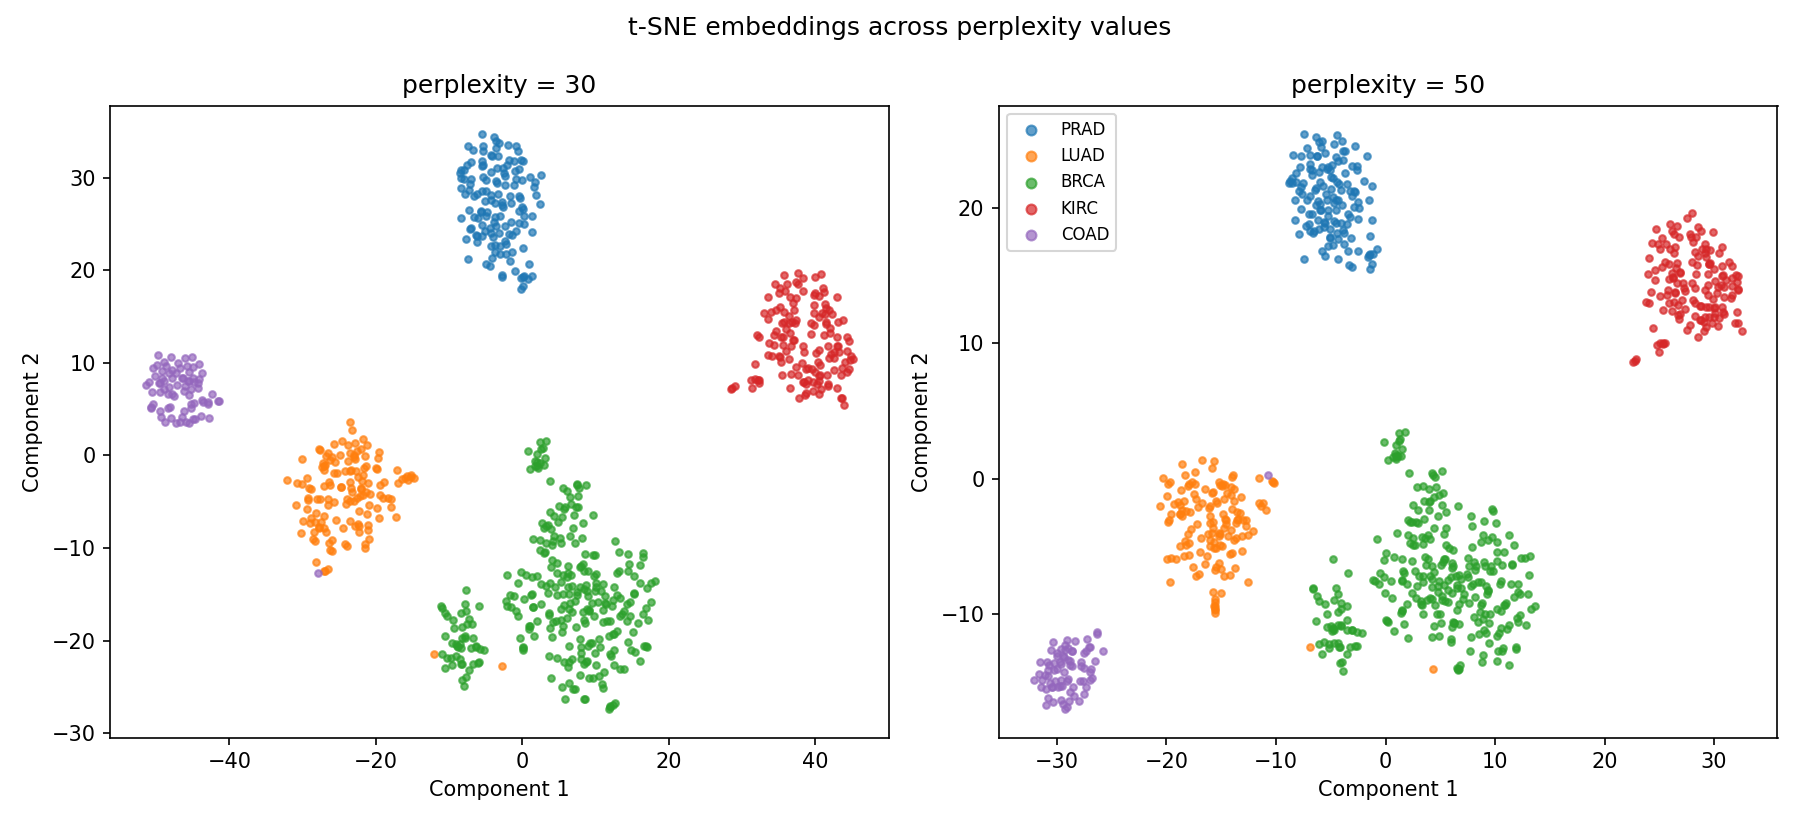
\includegraphics[width=\textwidth]{../figures/tsne_comparison.png}
\caption{t-SNE 2D embeddings at perplexity $30$ (left) and $50$ (right)
(reproduced from Phase 3), both PCA-preprocessed to 50 dimensions. Five
near-completely-separated clusters emerge at both settings, in direct
contrast to the muted linear separation achievable from the first three
raw principal components (Phase 3, Section~4.1).}
\label{fig:tsne}
\end{figure}

The Marchenko--Pastur spectral analysis (Figure~\ref{fig:spectral})
supplies independent confirmation from a fourth angle: the $27$ spectral
outliers identified against the random-matrix null are, by construction,
exactly the linear directions in the top-$2{,}000$-gene subset that a pure
noise matrix of matching shape could not produce -- i.e., the directions
carrying real biological signal. That this count sits in the same
single-digit-to-low-double-digit range as $D_2$ and the $k$-NN MLE mean,
despite being computed by an entirely different (global, eigenvalue-based,
random-matrix-theoretic) method on a differently pre-filtered feature set,
is strong triangulating evidence that the manifold's genuine degrees of
freedom number in the tens, not the hundreds implied by unfiltered global
PCA.

\begin{figure}[H]
\centering
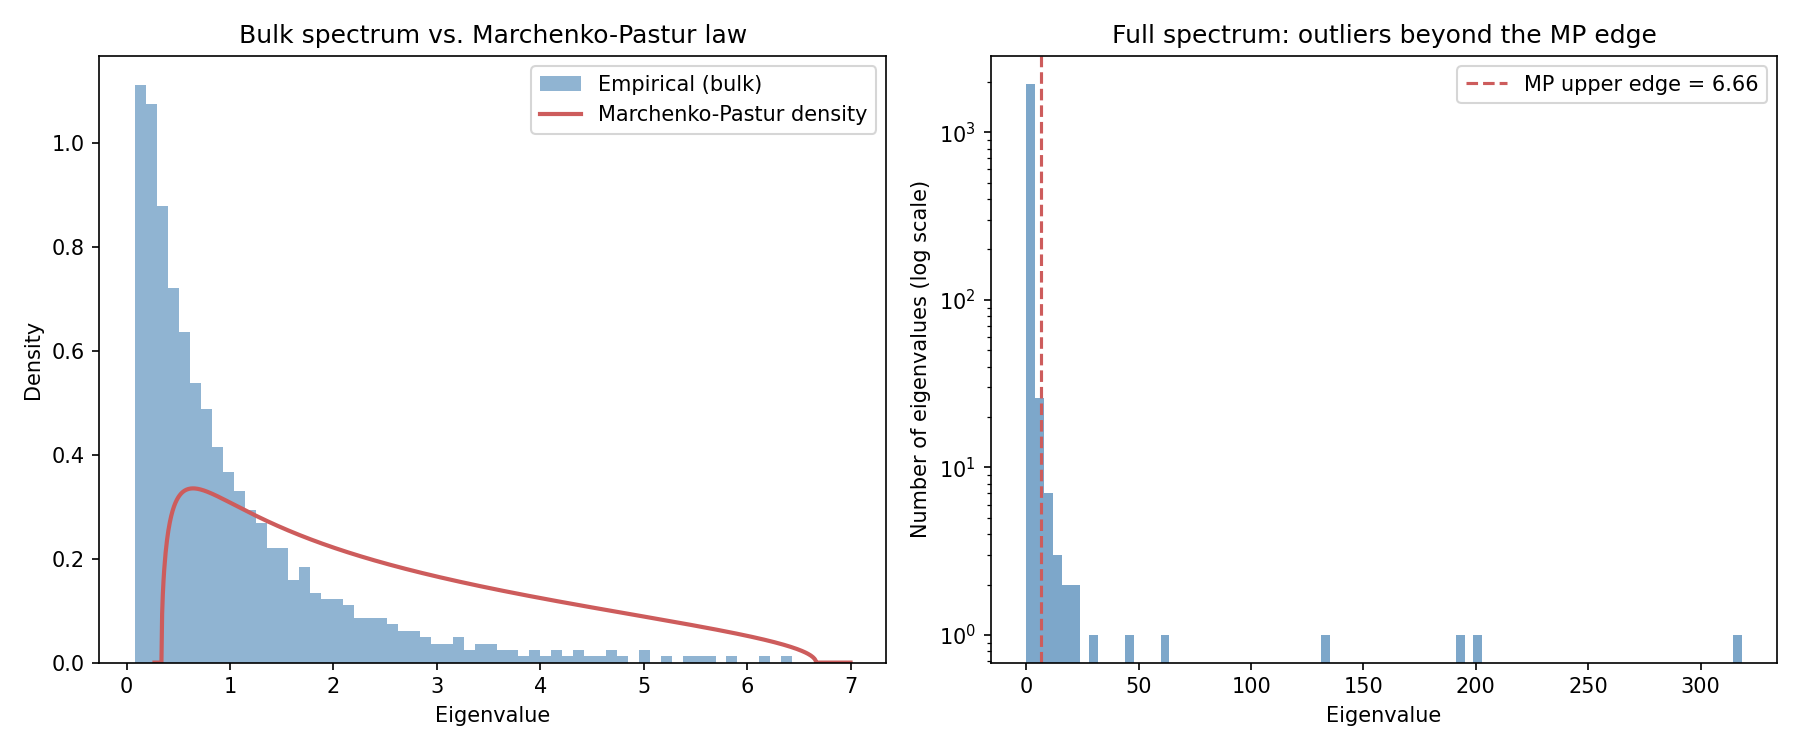
\includegraphics[width=\textwidth]{../figures/spectral_overlay.png}
\caption{Empirical spectrum of the top-$2{,}000$-gene correlation matrix
against the Marchenko--Pastur theoretical density (reproduced from Phase
3). Left: bulk eigenvalues within the theoretical support $[0.337, 6.657]$
overlaid with the theoretical density. Right: full spectrum on a log-count
axis, showing $27$ outlier eigenvalues (up to $318.3$) far beyond the
theoretical edge (dashed line) -- a fourth, independent estimate of the
manifold's signal dimensionality that agrees in order of magnitude with
$D_2$ and the $k$-NN MLE mean.}
\label{fig:spectral}
\end{figure}

\section{Consolidated Summary Table}
\label{sec:summary-table}

Table~\ref{tab:consolidated} consolidates every quantitative diagnostic
computed in Phases 1--3: ambient and analysis dimensionality, all three
intrinsic-dimension estimators (real data vs.\ both synthetic baselines),
PCA variance cutoffs and elbow criteria, Johnson--Lindenstrauss empirical
distortion against the theoretical bound, the Marchenko--Pastur spectral
outlier count, and the Mahalanobis-flagged outlier count. Entries marked
``--'' were not computed for the synthetic baselines in Phase 3: the
Johnson--Lindenstrauss, spectral, and Mahalanobis diagnostics were run only
on the real dataset and the top-$2{,}000$-gene subset derived from it,
since their purpose (testing whether \emph{this specific, biologically
structured} dataset departs from random-matrix/i.i.d.\ expectations) is not
meaningful to repeat on a matched Gaussian-noise or linear-manifold
baseline that has no biological structure to test against; this is a
scope decision inherited from Phase 3, stated there explicitly, and not an
omission.

\begin{table}[H]
\centering
\caption{Consolidated high-dimensional geometric diagnostics across the
real TCGA Pan-Cancer dataset and Phase 2's two synthetic calibration
baselines (matched in shape to $n=801$, $d=20{,}264$).}
\label{tab:consolidated}
\begin{tabular}{lccc}
\toprule
\textbf{Metric / Estimator} & \textbf{TCGA PANCAN} & \textbf{Gaussian Noise} & \textbf{Linear Manifold} \\
\midrule
Ambient dimension $d$ (raw, pre-filter) & 20{,}531 & -- & -- \\
Analysis dimension $d$ (post zero-var.\ filter) & 20{,}264 & 20{,}264 & 20{,}264 \\
True intrinsic dimension (by construction) & unknown & $\approx d$ (none) & 5 \\
Correlation dimension $\hat D_2$ ($R^2$) & 7.73 (1.000) & 419.52 (1.000) & 4.29 (1.000) \\
$k$-NN MLE mean, $k \in \{5,10,20\}$ & 29.36 & 610.36 & 5.44 \\
\quad$k$-NN MLE ($k=5$) & 33.16 & 626.09 & 5.69 \\
\quad$k$-NN MLE ($k=10$) & 29.55 & 621.67 & 5.42 \\
\quad$k$-NN MLE ($k=20$) & 25.37 & 583.31 & 5.20 \\
Kaiser-criterion PCA elbow (components) & 100 & 386 & 5 \\
Curvature-criterion PCA elbow (components) & 3 & 54 & 5 \\
PCA components for 90\% variance & 392 & 688 & 5 \\
PCA components for 95\% variance & 548 & 742 & 5 \\
PCA components for 99\% variance & 732 & 788 & 5 \\
MP spectral outlier count (top-2,000 genes, $\gamma=2.500$) & 27 & -- & -- \\
JL target dimension $k$ ($\varepsilon=0.2$, Eq.~\ref{eq:jl-recap}) & 1{,}543 & -- & -- \\
JL empirical mean distortion $\bar\rho$ & 0.9996 & -- & -- \\
JL max $|\rho - 1|$ (theoretical bound: $0.2$) & 0.0808 & -- & -- \\
JL fraction of pairs within $(1\pm\varepsilon)$ bound & 100\% & -- & -- \\
Mahalanobis-flagged outliers ($\alpha=0.025$, $\mathrm{df}=800$) & 0 & -- & -- \\
\bottomrule
\end{tabular}
\end{table}

\noindent where the Johnson--Lindenstrauss target dimension is
\begin{equation}
k \geq \frac{4 \ln n}{\varepsilon^2/2 - \varepsilon^3/3}
\label{eq:jl-recap}
\end{equation}
(Dasgupta--Gupta, 1999; Phase 3, Eq.~1), evaluated here at $n=801$,
$\varepsilon=0.2$.

Every row of Table~\ref{tab:consolidated} that is populated for all three
datasets shows the same qualitative pattern: the Gaussian-noise baseline
sets a ceiling (correlation dimension near the ambient dimension itself,
$k$-NN MLE in the hundreds, hundreds of PCA components needed for any
variance threshold, since isotropic noise has no compressible structure),
the linear-manifold baseline recovers its known ground truth of $5$ almost
exactly across every estimator once the noise level is correctly calibrated
(Phase 2, Section~4.5), and the real data sits strictly between these two
extremes, but far closer to the manifold baseline's regime than to the
noise baseline's -- direct, calibrated evidence that the Pan-Cancer
expression manifold is genuinely low-dimensional rather than
high-dimensional noise with superficial class labels. The rows populated
only for the real dataset (Johnson--Lindenstrauss, spectral outliers,
Mahalanobis) each independently confirm a different piece of the same
picture: distances survive an aggressive $13.1\times$ random-projection
compression almost perfectly ($\bar\rho = 0.9996$), the correlation
structure contains $27$ directions no random matrix of matching shape could
produce, and not a single sample registers as a formal multivariate outlier
under Ledoit--Wolf-regularized Mahalanobis distance at the chosen
threshold -- a finding discussed critically, not uncritically, in
Section~\ref{sec:limitations}.

\section{Methodological \& Theoretical Limitations}
\label{sec:limitations}

\subsection{Small Per-Class Sample Sizes}

The five cancer types are unevenly represented: BRCA accounts for
$300$ of $801$ samples ($37.45\%$) while COAD accounts for only $78$
($9.74\%$, Phase 1, Table~2). Every class-conditional or cross-referenced
claim made in this project -- the visual cluster-purity assessment in
Phase 3, the class breakdown of the ten most-extreme Mahalanobis-distance
samples (4 BRCA, 3 LUAD, 3 KIRC, $0$ PRAD/COAD, Phase 3, Table~7) -- carries
substantially more sampling uncertainty for COAD than for BRCA. With
$n_{\text{COAD}} \approx 78$, any claim of the form ``COAD samples are/are
not disproportionately represented among outliers'' has wide confidence
intervals under a binomial or hypergeometric null and should not be
over-interpreted; the absence of COAD samples in the top-10 most-extreme
list in Phase 3 is at least partially explained by COAD's small class
share alone ($9.74\%$, so $\approx 1$ COAD sample is expected in a random
top-10 by chance), independent of any true underlying difference in
Mahalanobis distance.

\subsection{Potential Technical Batch Effects}

TCGA Pan-Cancer data are aggregated across dozens of contributing sequencing
centers, processed over a period of years, using instrument and
sample-preparation protocols that were not held constant across
submissions. No batch/center covariate is present in this Kaggle-mirrored
release of the dataset, so it is impossible to directly test for or correct
batch effects here. This is a material caveat for every geometric claim in
Phases 2--3: sequencing-depth normalization differences, reagent-lot
effects, or center-specific processing pipelines could contribute
systematic, non-biological variance that a purely unsupervised geometric
analysis cannot distinguish from genuine cancer-type signal. Given that
cancer type is almost certainly correlated with submission center (tissue
of a given type is disproportionately collected and sequenced at
specialized centers), some fraction of the very clean t-SNE/UMAP cluster
separation observed in Phase 3 may be inflated by a batch-cancer-type
confound rather than reflecting cancer-type biology in isolation. This does
not invalidate the intrinsic-dimension estimates -- batch effects are
themselves a lower-dimensional, systematic source of variance, and would if
anything tend to \emph{reduce}, not inflate, the estimated intrinsic
dimension by adding additional coherent (low-rank) structure -- but it does
mean that ``intrinsic dimension of the tumor manifold'' as measured here
should be read as ``intrinsic dimension of the tumor-plus-processing-batch
manifold,'' a distinction that cannot be resolved without batch metadata
this dataset does not provide.

\subsection{i.i.d.\ Violations from Gene Co-expression Networks}

The Marchenko--Pastur law (Phase 3, Eq.~3) and the Laurent--Massart
concentration bound (Phase 3, Eq.~5) both assume, in their classical form,
i.i.d.\ (or at minimum uncorrelated) coordinates. Genes are not
independent: they are organized into co-expressed regulatory pathways and
modules with strong pairwise and higher-order correlations, which is
precisely the biological signal this entire project is trying to detect.
This is why Phase 3's own results depart from the i.i.d.\ null in exactly
the two ways theory predicts a correlated system would: (1) the $27$
Marchenko--Pastur spectral outliers are a direct measurement of departure
from an i.i.d.\ null, not a modeling failure -- a genuinely unstructured
$2{,}000$-gene random matrix of the same shape would show none; and (2) the
distance-concentration ratio plateaus around $\approx 5$ at large feature
counts rather than continuing to shrink toward the near-certain
concentration ($1.81\times10^{-20}$ tail probability) the i.i.d.\ Gaussian
bound implies at $d=20{,}264$ (Phase 3, Table~4) -- correlated coordinates
do not average away independently, so the effective number of ``free''
directions driving pairwise distance is smaller than $d$ itself, which
directly slows concentration relative to the i.i.d.\ rate. Both departures
are therefore reported as findings, consistent with the project's
constraint against silently correcting or hiding disagreement between
theory and data; they do mean that any \emph{quantitative} probability
computed from these bounds (e.g., the $1.81\times10^{-20}$ tail bound
itself) should be read as a qualitative benchmark for an idealized null,
not a calibrated statement about this correlated dataset.

\section{Future Work \& Methodological Improvements}
\label{sec:future-work}

Given additional time and compute budget, the following extensions would
most directly strengthen the project's conclusions:

\begin{itemize}
  \item \textbf{Bootstrap stability selection for correlation dimension.}
  Phase 2 notes that the automatically detected scaling region for $D_2$ on
  the real data is narrow ($5$ points, $r \in [149.6, 156.5]$), so the
  reported $R^2 = 1.000$ of the local linear fit does not itself capture
  finite-sample uncertainty in \emph{which} scaling region is selected.
  Repeating the full correlation-dimension pipeline (radius-quantile
  estimation, automatic scaling-region detection, slope fit) across, e.g.,
  $200$ bootstrap resamples of the $801$ patients would yield a confidence
  interval on $D_2$ rather than a point estimate, and would additionally
  reveal whether the scaling-region \emph{location} itself is stable across
  resamples or an artifact of this particular sample.
  \item \textbf{Non-linear shrinkage covariance estimation.} Section
  \ref{sec:summary-table} and Phase 3's discussion both attribute the
  zero-Mahalanobis-outlier result partly to Ledoit--Wolf's isotropic
  shrinkage target ($\mu I$) compressing distances non-uniformly across a
  spectrum ranging from near-zero to $318.3$. Ledoit and Wolf's later
  non-linear shrinkage estimator (2017, quadratic-inverse shrinkage),
  which fits a smooth, eigenvalue-dependent shrinkage function rather than
  a single scalar intensity $\alpha$, would shrink small and large
  eigenvalues by different amounts and is the natural next step for
  testing whether the null Mahalanobis result is a genuine finding or a
  consequence of the specific (linear) shrinkage target used here.
  \item \textbf{Batch-effect correction and sensitivity analysis.} Given
  the concern raised in Section~\ref{sec:limitations} about unmodeled
  TCGA submission-center effects, obtaining center/batch metadata (from the
  original TCGA/GDC portal rather than this Kaggle mirror) and applying a
  standard batch-correction method (e.g., ComBat, Johnson et al., 2007)
  prior to re-running the full Phase 2--3 pipeline would directly test how
  much of the observed cluster separation and intrinsic-dimension estimate
  is attributable to processing batch versus tumor biology.
  \item \textbf{Curved (nonlinear) manifold calibration baseline.} Phase
  2's linear-manifold baseline validates estimator recovery of a
  \emph{flat} $5$-dimensional ground truth only. Given Section
  \ref{sec:synthesis}'s argument that the real manifold is likely curved
  (explaining why PCA needs far more components than $D_2$ or the $k$-NN
  MLE suggest), a third synthetic baseline -- e.g., points on a known
  low-dimensional curved manifold (a Swiss roll or S-curve) embedded with
  matched noise in $\mathbb{R}^{20{,}264}$ -- would let every estimator's
  behavior under \emph{curvature} be calibrated directly, rather than
  inferred indirectly as in Section~\ref{sec:synthesis}.
  \item \textbf{Permutation-calibrated Mahalanobis threshold.} The
  $\chi^2_{800}$ threshold (correctly set at the rank of the estimator,
  $\mathrm{df}=n-1=800$, rather than the feature count $p=2{,}000$) still
  assumes asymptotic multivariate normality of $D^2$. Because the mean and
  covariance used to score each sample are estimated from the same $801$
  samples being scored, the exact reference distribution is a scaled Beta
  rather than a $\chi^2$ at any degrees of freedom, and shrinkage perturbs
  it further. A permutation-based null (recomputing $D^2$ under
  row-shuffled or resampled data to build an empirical threshold) would
  replace this asymptotic approximation with a threshold calibrated
  directly against this dataset's own shrinkage-distorted distribution.
\end{itemize}

\section{Conclusion}

Across four independent estimators and two calibrated synthetic baselines,
this project finds the TCGA Pan-Cancer expression manifold's genuine,
curvature-aware degrees of freedom to be in the range of roughly $7$ to
$30$ -- three orders of magnitude below the ambient dimension $d=20{,}531$
-- while showing explicitly why a naive linear-PCA measure of ``dimension
needed for visual separation'' reports a much larger number ($100$--$392$
components): linear methods must spend components unfolding curvature that
local, nonlinear-aware estimators see through directly. This reconciliation,
not any single number in isolation, is the project's central technical
finding, and is corroborated independently by both the nonlinear
embeddings (Phase 3) recovering near-perfect five-cluster structure from
the same underlying $50$-dimensional linear substructure, and by the
Marchenko--Pastur spectral analysis identifying $27$ outlier eigenvalues in
close numerical agreement with the local estimators despite resting on
entirely unrelated (random-matrix-theoretic) machinery.

\section{References}

\begin{itemize}
\item Grassberger, P., \& Procaccia, I. (1983). Measuring the strangeness
of strange attractors. \emph{Physica D}, 9(1-2), 189--208.
\item Levina, E., \& Bickel, P. J. (2004). Maximum likelihood estimation
of intrinsic dimension. \emph{Advances in Neural Information Processing
Systems}, 17.
\item Johnson, W. B., \& Lindenstrauss, J. (1984). Extensions of Lipschitz
mappings into a Hilbert space. \emph{Contemporary Mathematics}, 26, 189--206.
\item Dasgupta, S., \& Gupta, A. (2003). An elementary proof of a theorem
of Johnson and Lindenstrauss. \emph{Random Structures \& Algorithms},
22(1), 60--65.
\item Marchenko, V. A., \& Pastur, L. A. (1967). Distribution of
eigenvalues for some sets of random matrices. \emph{Mat. Sb.}, 114(4), 507--536.
\item Ledoit, O., \& Wolf, M. (2004). A well-conditioned estimator for
large-dimensional covariance matrices. \emph{Journal of Multivariate
Analysis}, 88(2), 365--411.
\item Ledoit, O., \& Wolf, M. (2017). Numerical implementation of the
QuEST function. \emph{Computational Statistics \& Data Analysis}, 115,
199--223.
\item Laurent, B., \& Massart, P. (2000). Adaptive estimation of a
quadratic functional by model selection. \emph{Annals of Statistics},
28(5), 1302--1338.
\item Johnson, W. E., Li, C., \& Rabinovic, A. (2007). Adjusting batch
effects in microarray expression data using empirical Bayes methods.
\emph{Biostatistics}, 8(1), 118--127.
\item van der Maaten, L., \& Hinton, G. (2008). Visualizing data using
t-SNE. \emph{Journal of Machine Learning Research}, 9, 2579--2605.
\item McInnes, L., Healy, J., \& Melville, J. (2018). UMAP: Uniform
Manifold Approximation and Projection for dimension reduction.
\emph{arXiv:1802.03426}.
\item Weinstein, J. N., et al. (2013). The Cancer Genome Atlas Pan-Cancer
analysis project. \emph{Nature Genetics}, 45(10), 1113--1120.
\item Dataset: Gene Expression Cancer RNA-Seq (TCGA Pan-Cancer HiSeq),
\url{https://www.kaggle.com/datasets/debatreyadas/gene-expression-cancer-rna-seq}.
\end{itemize}

\appendix
\section{Appendix A: AI Usage Log}
See \texttt{ai\_usage\_log.md} in the repository root for the full,
incrementally maintained log, including the Phase 4 entry documenting the
generation of this report and its consolidated table.

\end{document}
